

%\documentclass{scrippsthesis}
\documentclass[a4paper,11pt,twoside]{UUthesis}
%\usepackage[pass]{geometry}
%%% HEADER INFORMATION %%%

\title{Network Traffic Simulator:  \\ Designing a flexible  Microscopic Traffic Management System using Python}
\author{Julia Ruiter}
\advisor{Yannis Velegrakis}
\reader{Ioana Hulpis}
\department{Department of Natural Sciences}

%%% Including new commands and packages.

% Allows for auto formatting of theorems,
% definitions etc.
\usepackage{amsthm}
\usepackage{graphics,graphicx}
\usepackage{tikz}
\usepackage{verbatimbox}
\usepackage{textgreek}
\usepackage[toc,page]{appendix}
\usepackage{float}
\usepackage{amsmath}


\newtheorem{thm}{Theorem}[chapter]
\newtheorem{lem}[thm]{Lemma}
\newtheorem{prop}[thm]{Proposition}
\newtheorem{cor}[thm]{Corollary}

\theoremstyle{definition}
\newtheorem{defn}[thm]{Definition}
\newtheorem{ex}[thm]{Example}

\theoremstyle{remark}
\newtheorem*{rmk}{Remark}
\newtheorem*{notn}{Notation}
\newtheorem*{pf}{Proof}

% Add any new commands here.
\newcommand{\Q}{\mathbb{Q}}
\newcommand{\Z}{\mathbb{Z}}
\newcommand{\F}{\mathbb{F}}
\newcommand{\R}{\mathbb{R}}
\newcommand{\NN}{\mathbb{N}}

%file path for images


%%%  END HEADER %%%

\begin{document}
%\begin{comment}

\frontmatter

\maketitle % Title page


%%%% ABSTRACT.
\begin{abstract} 
[write text here]]
\end{abstract}

%%% ACKNOWLEDGEMENTS.
\begin{acknowledgments}
I'm extremely grateful for my partner, Warren Fletcher, for all the support he has provided me (both professionally and emotionally) in the duration of both thesis and this entire master's program. He has given invaluable guidance in writing and designing a proper/professional piece of software, and has patiently helped fill in the gaps in my computer science knowledge, pointing me in the right direction for data structure and algorithm usage.
\end{acknowledgments}

%%% CONTENTS, FIGURES, TABLES
\tableofcontents
\listoffigures
%\listoftables

%%% End of the front matter.

%% MAIN MATTER - INCLUDE THE CHAPTERS.
\mainmatter

% CHAPTERS %
\chapter{Introduction}
\chapter{Lorenz, Liu, and Other Chaotic Systems}

\par Thanks to $\it{Jurassic Park}$, most everyone is familiar with the idea of the ``Butterfly Effect'':  the idea that one small perturbation in the present can set the future on a wildly different course.  This idea comes from Ed Lorenz, chaos theory's pioneer, and his observations of dynamical systems with strange attractors, that is, systems of equations that have an element of chaos built into them.  These systems are a part of the family of Lorenz equations and are of the following form:
%
\begin{equation}
\begin{cases} 
\dot{x} = \sigma(y-x) \\ 
\dot{y} = rx - y - xz \\ 
\dot{z} = xy - bz
\end{cases}
\end{equation}
%
%Figure \ref{fig:genLorenz} original Lorenz system
%  use math mosde $_$ for all variables in paragraphs
where the dot denotes the first time derivative of each variable, and with the Prandtl number ($\sigma$), Rayleigh number($r$), and $b$ all greater than 0.  The aperiodic nature of this system defined by a total lack of fixed points and quasiperiodic orbits for any initial trajectory means that the outcome is very sensitive to its initial conditions.  The deterministic nature of the system, the fact that its irregularity comes not from randomness, but the nonlinear relationships of variables, means that once the initial conditions have been set, the outcome at any given time $t_0$ is always going to give the same values $x$, $y$, $z$.  These two attributes make the Lorenz equations a very good candidate for an encryption system (more on that in the next chapter).  

\begin{figure}[H]
    \centering
	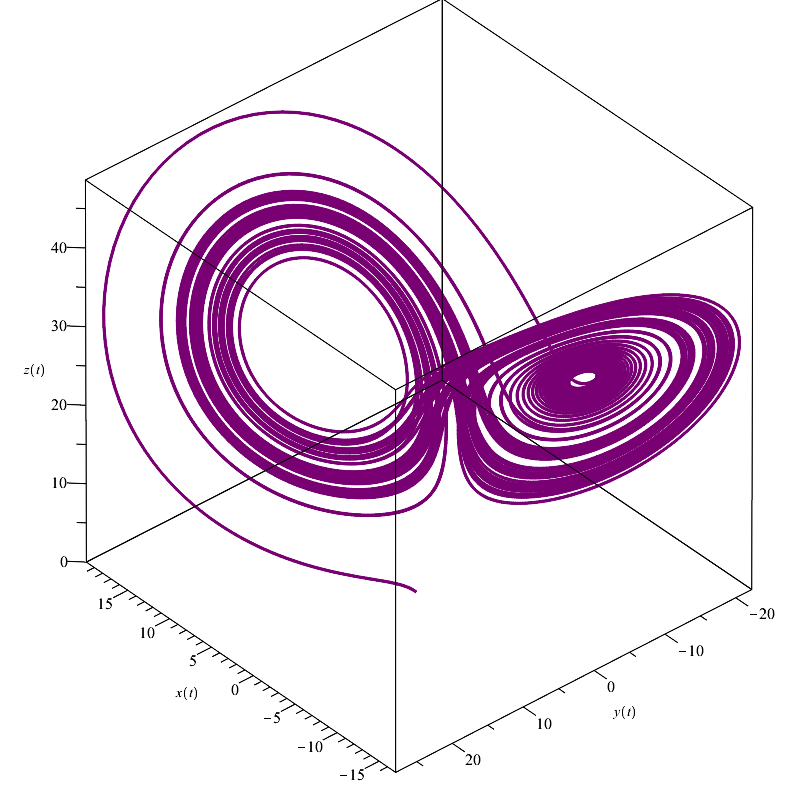
\includegraphics[width=\linewidth]{Figures/lorenz2.PNG}
	\caption{Lorenz System where $r = 28, \sigma = 10, and b = 8/3$. *}
	\label{fig:genLorenz}
\end{figure}

\par In other words, chaotic systems have a dense orbit, meaning that the system has at least two orbits that are sensitive to the initial conditions, thus excluding systems with only one cycle as well as systems consisting of just an equilibrium point which are systems with clear orbits in their phase space (to be defined in glossary). 

\par The most notable feature of the Lorenz systems is that it contains a strange attractor.  An attractor is a subset A of the system's phase space where the neighborhood of A is defined as being the basin of attraction, the basin of attraction being the region of phase space where the system starts to show cyclic action, usually resulting in a stable orbit, or condensing towards a point.  Strange attractor differ, however, in that given any two points arbitrarily close to each other in one orbit, several orbits later will be arbitrarily further away, rather than same or closer.  It is this quality that makes the system chaotic.

\par What is important to note, though, is that not all values of $r$, $b$, and $\sigma$ will yield a chaotic system. An analysis of the bifurcation diagrams (a diagram that shows values for which there are stable and unstable equillibria) of $r$ help explain why only certain values work.

\par for Lorenz systems, there is always an equilibrium at the origin $(0,0,0)$, this is true of any variation of the Lorenz system, using any values $b$, $r$, and $\sigma$.  However, if $r>1$, then other critical points appear:
%
\begin{equation}
(\sqrt{b(r-1)},\sqrt{b(p-1)},(r-1))
\end{equation}
\begin{equation}
(-\sqrt{b(r-1)},-\sqrt{b(p-1)},(r-1))
\end{equation}
%
which means the system exhibit cyclical behaviour if and only if $r$ and $\sigma$ are positive and have the property that:
%
\begin{equation}
\sigma > b + 1 
\end{equation}
\begin{equation}
r > \sigma \frac{\sigma + b + 3}{\sigma - b - 1}
\end{equation}
%
because of that, the original version of the Lorenz system (and the one used later in this text) is usually restricted to values close to:
\begin{equation}
\begin{cases} 
r = 28 \\ 
b = \frac{8}{3} \\ 
\sigma = 10
\end{cases}
\end{equation}
%
which are the original set of values that Lorenz accidentally discovered that exhibited chaotic behaviour.

\par What happens if the variables don't all fall in this range?  Take this example where only the value of \textsigma has been altered:
%
\begin{figure}[H]
    \centering
	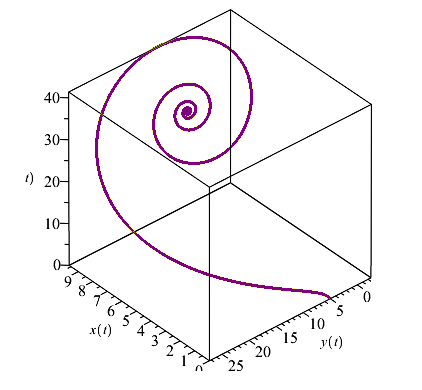
\includegraphics[width=\linewidth]{Figures/lorenz_s2.png}
	\caption{Lorenz System where $r = 28, \sigma = 1, and b = 8/3$}
	\label{fig:badLorenz}
\end{figure}
%Figure \ref{fig:badLorenz} nonchaotic Lorenz system
%
As you can see, the resulting graph is not at all chaotic, with x, y, and z all having a fixed limit (regular attractor) as time goes to infinity, or otherwise exhibiting standard actions as dynamical system.  This means that distance between two points at t0 will always be larger than the distance between those points at a later $t_1$, meaning that it is easy to predict how the system behaves over time.  Because of the predictability, a Lorenz system with these parameters cannot be used to encrypt information, as values follow a predictable pattern.  For that reason, we will only consider Lorenz systems with chaotic action (like those mentioned at the beginning of the chapter) as candidates for strong encryption.

%
\subsection{Liu and Chen Systems}

\par Lorenz systems are not the only type of dynamical system that exhibit this sort of chaotic behaviour.  Two other systems, Liu and Chen, are variations of the Lorenz system, with slightly different dependencies and thus different usable chaotic parameters.

\par Although it is a bit difficult to see, the Chen and Liu systems actually shows greater levels of chaos that the Lorenz system, and thus are better candidates for chaotic encryption.  Because of this, these systems, though only discovered in the past 15 years,  are most often used and referenced in current publications in this field.

\par Take the Chen system:
%
\begin{equation}
\begin{cases} 
\dot{x} = a(y - x) \\ 
\dot{y} = (c - a)x + cy + xz \\
\dot{z} = xy - bz
\end{cases}
\end{equation}
%
\par 

%


%\end{equation}
% backslash square bracket to start equation
% \cite to cite in text
% tex will not display sources that are not refrenced ==> FIXED with nocite
\chapter{Softare Structure}
\label{Structure}

\par This software is comprised of several interconnected modules.  Each module represents an abstract concept required for modelling a traffic scenario, each containing as many classes as are needed to create the components necessarily for that concept.  This results in the creation of three self\-contained modules representing the network, the cars/objects traversing the network, and the state-changer.  To make the simulation complete and fully self-contained, the user may utilize two additional optional modules for generating the network structure and car objects. Following normal naming conventions, and module that a user may directly interact with has been named using capitalization; dependent modules (hidden to the user) are named using only lowercase.

\section{Essential Modules for the Network Traffic Simulator}

\subsection{Network Module:  traffic\_network}

\par As noted in the previous chapter, a network must have three components (network structure, nodes, and edges) \textit{and} there exists an inherent hierarchy to these structures (a network only exists by defining sets of connected nodes).  Though for creation purposes it may make sense to define the nodes and edges and let the network be a dependent object, that does not make sense for the problem at hand:  traffic simulation is the analysis of objects moving over a network, therefore the Network itself must be given (requiring a class of its own), leading to Nodes and Edges being dependent classes.  The module \textbf{traffic\_network} has been created to collect the instances and interactions of all network components for a simulation instance.  \\

\par The resulting module structure is as follows:

\begin{figure}[H]
    \centering
	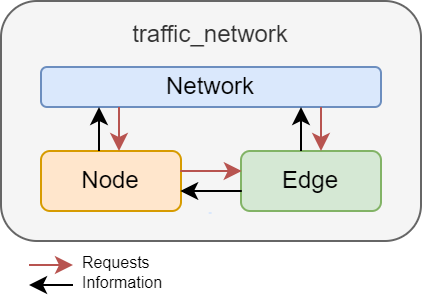
\includegraphics[width=0.5\textwidth]{tex files/Figures/traffic_network_module.png}
	\caption[Network Module:  traffic\_network]{Hierarchical structure of classes within the traffic\_network module.  Directions of requests and information flow between classes is depicted by colored arrows }
	\label{fig:network_module}
\end{figure}


\subsection{Car Module:  network\_cars}

\par "Car" is the general term I use to describe an object traversing the network as it allows for intuitive labeling of its attributes.  Once instantiated, a car is not dependent on the network to continue existing; to represent this semi-independence, the Car class was moved to a separate module:

\begin{figure}[H]
    \centering
	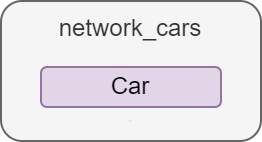
\includegraphics[width=0.3\textwidth]{tex files/Figures/car_module.png}
	\caption[Car Module:  network\_cars]{Classes structure within the network\_cars module}
	\label{fig:cars_module}
\end{figure}

\par In practice, though, the car is not very interesting when trying to simulate overall network behavior and ensuing traffic scenarios.  Any attributes the user may care about (such as current location) are only relevant in context.  So while \textbf{network\_cars} technically exists as a self-contained module, it is never used in isolation.  Instead, this module is automatically imported into the \textbf{traffic\_network} module, seamlessly allowing these two modules to interact with one another.


\subsection{State Module:  Traffic}

\par The final component necessary to creating a simulation  is a mechanism for advancing the state of the network.  State changing includes adding, removing, and advancing any cars on the network as far as possible within a particular unit of time, and are all essential for creating a hands-off simulation. \\

\par But simulation state refers to more than the set of current car locations.  It includes system metadata (like lists of nodes and edges in a network, and their attributes) and dependent calculations from that metadata.  By allowing the user an access point to adapt any component of the network, this software achieves its goal of being adaptable and extensible to other types of networks and simulations.  \\

\par The Traffic modules serves as an API to the underlying simulation, allowing users to (indirectly) interact with the network components and car objects.  The set of all these access points into the simulation allows for the direct management of traffic and has thus been wrapped into an aptly named class,  \textbf{TrafficManager}:

\begin{figure}[H]
    \centering
	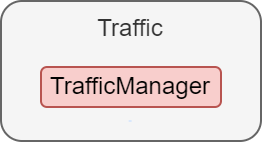
\includegraphics[width=0.3\textwidth]{tex files/Figures/traffic_manager_module.png}
	\caption[State Module:  Traffic\_cars]{Classes structure within the Traffic module}
	\label{fig:traffic_module}
\end{figure}


\noindent  Note that the \textbf{Traffic} module allows only for indirect access to the simulation components.  By using this API as an intermediary between users and network simulation components, the user is given access only to commands that are relevant to analysis, and hide internal functions that facilitate those actions.  For example, if a user wants a particular car to halt in place, they can call on the API function that requests it.  The \textbf{Traffic} module then passes that request to the \textbf{traffic\_network} and/or \textbf{network\_cars} module to handle if and when it becomes relevant.


\section{Essential Module Interaction}

\par Putting the modules together, we get the following depiction of how the modules interact with one another:

\begin{figure}[H]
    \centering
	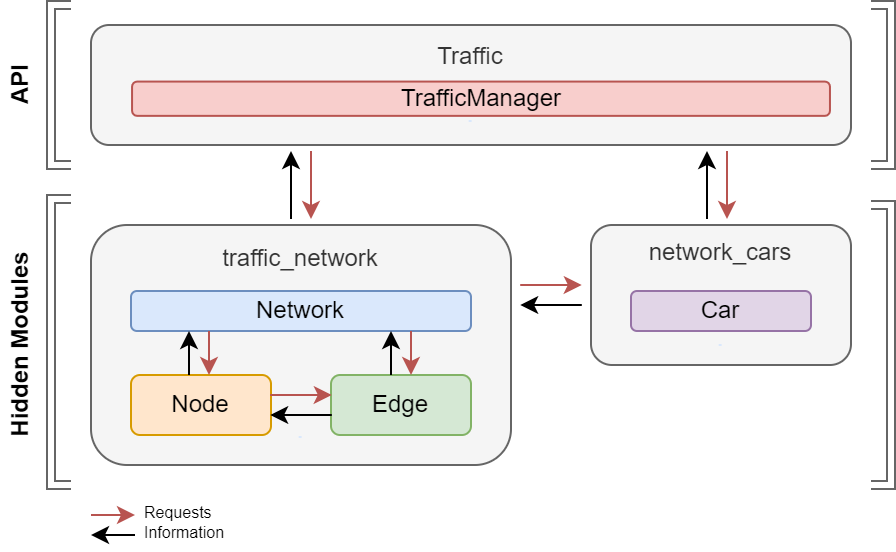
\includegraphics[width=0.9\textwidth]{tex files/Figures/detailed_essentials.png}
	\caption[Software Interaction:  Full View]{Full view of interactions between the modules and their individual components}
	\label{fig:interactions_detailed}
\end{figure}

\noindent  However, as the user doesn't need to concern themselves with the specifics on which functions in which classes work and when, we can streamline the architecture diagram to:

\begin{figure}[H]
    \centering
	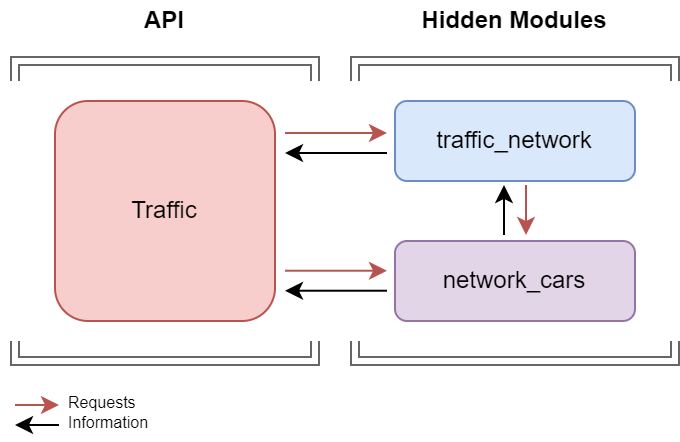
\includegraphics[width=0.7\textwidth]{tex files/Figures/simplified_essentials.png}
	\caption[Software Interaction:  User View]{Generalized overview of interactions between modules}
	\label{fig:interactions_simplified}
\end{figure}



\section{Extended Module Interaction}

Two optional additional modules for generating the underlying network and the car objects themselves can be integrated into the 
% \usetikzlibrary{positioning,matrix,shapes.arrows}

% \tikzset{
%   modulematrix/.style={draw=blue!50!red,rounded corners,matrix of nodes,row sep=1cm,column sep=1cm,nodes={draw=green!70,align=center,font=\sffamily},inner ysep=0.5cm},
%   module/.style={rounded corners, align=center, font=\sffamily, thick},
%   simple module/.style={module, top color=blue!10, bottom color=blue!35, draw=blue!75, text width=40mm, minimum height=15mm},
%   module down arrow/.style={module arrow, shape border rotate=-90},
%   module right arrow/.style={module arrow},
% module arrow/.style={single arrow, single arrow head extend=2.5mm, draw=gray!75, inner color=gray!20, outer color=gray!35, thick, shape border uses incircle, anchor=tail,minimum height=0.7cm},
% }

% \begin{tikzpicture}
% \node [simple module] (mA) {Item-1};
% \matrix[modulematrix,below=of mA,label={[anchor=south]below:Item-2}] (mB) {Item-3 & Item-4 \\};
% \matrix[modulematrix,right=of mB,nodes={text width=5cm,align=center},label={[anchor=north]above:Module C}] (mC) {Item-5 \\ Item-6 \\};
% \matrix[modulematrix,below=of mC,label={[anchor=south]below:Item-9}] (mD) {Item-7 & Item-8 \\};

% \foreach \n in {mA,mC-1-1,mC,mD}
%   \node[module down arrow,below=1mm of \n] {};

% \foreach \n in {mB-1-1,mB,mD-1-1}
%   \node[module right arrow,right=1mm of \n] {};
% \end{tikzpicture}

%\end{comment}


%%% End of the main matter.
\backmatter

%%%% BIBLIOGRAPHY (Be sure cto compile with BibTeX to make this work!)
%
\nocite{*} % Show everything in bib file, not just things that are explicitly cited.
\bibliography{bibliography}
\bibliographystyle{alpha}
%\printbibliography


\end{document}

% double check/cross with original doc--might be undoing what is going on in 
% have to bibtex bibliography first, then can tex rest of file